\begin{pastexam}[label={px:ntu-108-dsaa-03}]{臺大資工所 108 學年度 第 3 題}
（問答）

(10\%) Draw the final min-heap tree after the following operations: insert 7, insert 4, insert 3,
insert 1, delete min, insert 9, insert 2, insert 5, delete min, delete min.
\end{pastexam}

\begin{pastsoln}
答案：最後的最小堆積是
\begin{center}
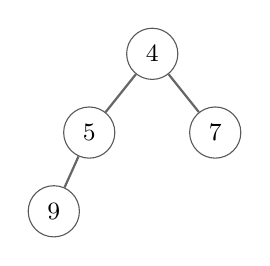
\begin{tikzpicture}[
    hn/.style={circle, draw=black!65, line width=0.4pt, minimum size=6.5mm, inner sep=0pt, font=\small},
    level distance=10mm, edge from parent/.style={draw=black!60, thick},
    level 1/.style={sibling distance=16mm}, level 2/.style={sibling distance=9mm}]
\node[hn] {4}
    child {node[hn] {5} child {node[hn] {9}} child[missing]}
    child {node[hn] {7}};
\end{tikzpicture}
\end{center}
用陣列寫是 $[4, 5, 7, 9]$（位置從 $1$ 開始）。

做法照資結書第~8.1~節，最大堆積的比較方向反過來：插入時新的鍵放在陣列最後，和父節點比，比
父節點小就交換，一路往上（上浮）；刪除最小值時拿掉根，把最後一個鍵搬到根，和兩個子節點中
較小的比，比它大就交換，一路往下（下沉）。 位置 $i$ 的父節點在 $\lfloor i/2 \rfloor$，子節點在
$2i$、$2i + 1$。 逐步追蹤（陣列從位置 $1$ 寫起）：
\begin{center}
\small
\begin{tabular}{lll}
\toprule
操作 & 過程 & 之後的陣列 \\
\midrule
insert 7 & 空堆積，放在位置 1 & $[7]$ \\
insert 4 & 放在位置 2；$4 < 7$，和父節點交換 & $[4, 7]$ \\
insert 3 & 放在位置 3；$3 < 4$，交換 & $[3, 7, 4]$ \\
insert 1 & 放在位置 4；$1 < 7$ 交換到位置 2；$1 < 3$ 交換到根 & $[1, 3, 4, 7]$ \\
delete min & 拿掉 $1$，$7$ 搬到根；子節點 $3, 4$ 較小的是 $3$，交換 & $[3, 7, 4]$ \\
insert 9 & 放在位置 4；$9 > 7$，不動 & $[3, 7, 4, 9]$ \\
insert 2 & 放在位置 5；$2 < 7$ 交換到位置 2；$2 < 3$ 交換到根 & $[2, 3, 4, 9, 7]$ \\
insert 5 & 放在位置 6；父節點是位置 3 的 $4$，$5 > 4$，不動 & $[2, 3, 4, 9, 7, 5]$ \\
delete min & 拿掉 $2$，$5$ 搬到根；子節點 $3, 4$，和 $3$ 交換； & \\
 & \quad 位置 2 的子節點 $9, 7$ 都比 $5$ 大，停 & $[3, 5, 4, 9, 7]$ \\
delete min & 拿掉 $3$，$7$ 搬到根；子節點 $5, 4$，和 $4$ 交換； & \\
 & \quad 位置 3 沒有子節點，停 & $[4, 5, 7, 9]$ \\
\bottomrule
\end{tabular}
\end{center}

三次 delete min 拿出來的依序是 $1, 2, 3$，正好是當時最小的鍵，可以順便核對：十個操作插入
$7, 4, 3, 1, 9, 2, 5$，刪掉 $1, 2, 3$，剩下 $\{4, 5, 7, 9\}$，最小的 $4$ 在根。 最後一步容易
畫錯的是 $7$ 搬到根以後該和誰交換：要和較小的子節點 $4$ 換。 和 $5$ 換的話根變成 $5$，它的
右子節點 $4$ 比它小，已經不是最小堆積。
\end{pastsoln}
